\apendice{Documentación técnica de programación}

\section{Introducción}

\section{Estructura de directorios}

\section{Manual del programador}

\subsection{API}
Para proveer los servicios de esta aplicación a nuevos entornos se incorpora una API para utilizar los diferentes servicios del sistema especificados en los Casos de Uso \ref{casos-uso}.

El funcionamiento general de la API serán peticiones \texttt{POST} mediante \texttt{application/x-www-form-urlencoded} ante rutas específicas con los datos requeridos para cada petición. Y según sea el caso el servidor contestará con un fichero \texttt{JSON} con la respuesta adecuada. De manera particular está el sistema en tiempo real que funciona mediante mensajes de \textit{WebSockets}\cite{wiki:websocket} usando la librería \textit{SocketIO}\cite{tool:socketio} mediante la serie de eventos de la Figura~\ref{fig:ws-secuence}

\begin{figure}
	\centering
	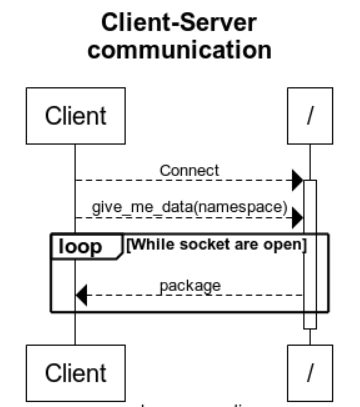
\includegraphics[width=0.7\textwidth]{img/ws-secuence.png}
	\caption{Comunicación cliente servidor \textit{websocket}}
	\label{fig:ws-secuence}
\end{figure}

Todas las respuestas del servidor contendrán los siguientes campos
\begin{lstlisting}[language=JSON]
{
  "status": 200|400|401|403|404|500,
  "message": "OK"|"Error description"
}
\end{lstlisting}

El valor de \texttt{status} tendrá un valor según los códigos HTTP definidos en el RFC 7231 y el mensaje será una explicación detallada del error producido.

Las distintas peticiones se especifican en la tabla \ref{tabla:api-specs2}
%\begin{table}[H]
%	\begin{center}
%		\begin{tabular}{p{0.095\textwidth} p{0.2\textwidth} p{0.37\textwidth} p{0.33\textwidth}}
%			\toprule
%			
%			\otoprule
%			
%			\bottomrule
%		\end{tabular}
%		\caption{Especificaciones del API}
%		\label{tabla:api-specs}
%	\end{center}
%\end{table}

\begin{center}\small
	\tablefirsthead{
		\toprule
		\textbf{CU}	&	\textbf{URI}	&	\textbf{Petición}	&	\textbf{Respuesta} \\
		\otoprule
	}
	\tablehead{
		\multicolumn{4}{l}{\small\sl continúa desde la página anterior}\\
		\toprule
		\textbf{CU}	&	\textbf{URI}	&	\textbf{Petición}	&	\textbf{Respuesta} \\
		\otoprule
	}
	\tabletail{
		\hline
		\multicolumn{4}{r}{\small\sl continúa en la página siguiente}\\
	}
	\tablelasttail{
		\hline
	}
	\bottomcaption{Especificaciones del API}
	\begin{xtabular}{p{0.095\textwidth} p{0.2\textwidth} p{0.37\textwidth} p{0.33\textwidth}}
		CU-1		&	\texttt{/api/auth}	& \begin{lstlisting}[language=JSONT]
"user": text,
"pass": text
\end{lstlisting}&\begin{lstlisting}[language=JSONT]
{
  ...,
  "token": text,
  "role": text,
  "username": text
}\end{lstlisting}
\\\hubu
CU-2.1  CU-4		&	\texttt{/api/beds}	& 
\begin{lstlisting}[language=JSONT]
"token": text
\end{lstlisting}
&
\begin{lstlisting}[language=JSONT]
...,
"beds": [{
  	"bed_name": text,
	"ip_group": text,
	"port": text,
	"MAC": text,
	"UUID": text
    }
    ...]
\end{lstlisting}
\\
CU-2.2		&	\texttt{/api/bed}	& 
\begin{lstlisting}[language=JSONT]
token=text&
bedname=text
\end{lstlisting}
&
\begin{lstlisting}[language=JSONT]
{
  ...,
  "namespace": text
}\end{lstlisting}
\\\hubu
CU-2.2		&	\texttt{/} \textit{(WebSocket)}	& 
\begin{lstlisting}[language=JSONT]
{
   "namespace": namespace
}
\end{lstlisting}
&
\begin{lstlisting}[language=JSONT]
{
  "results": [result, prob, press_state, hr_state],
  "instance": datetime
  "vital": [HR,RR,SV,HRV,B2B],
  "pressure": [P1,P2,..,P6] 
}\end{lstlisting}
\\\hubu
CU-3		&	\texttt{/api/users}	& 
\begin{lstlisting}[language=JSONT]
token=text
\end{lstlisting}
&
\begin{lstlisting}[language=JSONT]
{
  ...,
  "users":[text,...,text]
}\end{lstlisting}
\\\hubu
CU-3.1		&	\texttt{/api/user/add}	& 
\begin{lstlisting}[language=JSONT]
token=text&
username=text&
password=text&
password-re=text
\end{lstlisting}
&
\begin{lstlisting}[language=JSONT]
{
  ...
}\end{lstlisting}
\\\hubu
CU-3.2		&	\texttt{/api/user/mod}	& 
\begin{lstlisting}[language=JSONT]
token=text&
username=text&
password=text&
password-re=text
[&pasword-old=text]
\end{lstlisting}
&
\begin{lstlisting}[language=JSONT]
{
  ...
}\end{lstlisting}
\\\hubu
CU-3.3		&	\texttt{/api/user/del}	& 
\begin{lstlisting}[language=JSONT]
token=text&
username=text
\end{lstlisting}
&
\begin{lstlisting}[language=JSONT]
{
    ...
}\end{lstlisting}
\\\hubu
CU-4.1		&	\texttt{/api/bed/add}	& 
\begin{lstlisting}[language=JSONT]
token=text&
bed_name=text&
ip_group=text&
port=text&
MAC=text&
UUID=text
\end{lstlisting}
&
\begin{lstlisting}[language=JSONT]
{
  ...
}\end{lstlisting}
\\
CU-4.2		&	\texttt{/api/bed/mod}	& 
\begin{lstlisting}[language=JSONT]
token=text&
bed_name=text&
ip_group=text&
port=text&
MAC=text&
UUID=text
\end{lstlisting}
&
\begin{lstlisting}[language=JSONT]
{
  ...
}\end{lstlisting}
\\\hubu
CU-4.3		&	\texttt{/api/bed/del}	& 
\begin{lstlisting}[language=JSONT]
token=text&
bed_name=text
\end{lstlisting}
&
\begin{lstlisting}[language=JSONT]
{
  ...
}\end{lstlisting}
\\\hubu
CU-4.4		&	\texttt{/api/bed/perm}	& 
\begin{lstlisting}[language=JSONT]
token=text&
mode=[info|change]
[&bed_name=text&
username=text]
\end{lstlisting}
&
\begin{lstlisting}[language=JSONT]
{
  ...,
  "permission":[
   {
    "username":text,
    "bed_name":text
   },
   ...
  ]
}\end{lstlisting}
\\\bottomrule
	\end{xtabular}
	\label{tabla:api-specs2}
\end{center}

\section{Compilación, instalación y ejecución del proyecto}

\section{Pruebas del sistema}
